\section{Introduction}

% Overview of PR
Phone recognition (PR) entails transcribing speech into phonetic units that capture the physical realization of sounds, independent of language-specific phonological constraints.
By preserving acoustic nuances often abstracted away by word- or phoneme-level models\footnote{
For example, \textit{tell} may be transcribed as \textipa{[t\super hE\textltilde]} in Mainstream American English and \textipa{[t\super hEl]} in Scottish English, while 
the phonemic form of \textit{tell} is consistently 
\textipa{/tEl/}.
}, PR provides a robust foundation for cross-lingual speech processing \citep{li2022asr2k, yusuyin2025whistle} and  downstream applications in clinical \citep{shriberg2025clinical, choi-etal-2025-leveraging} and educational settings \citep{tu2018l1pronunciation, inceoglu2023l2assessment}.


\begin{figure}[t]
\centering
  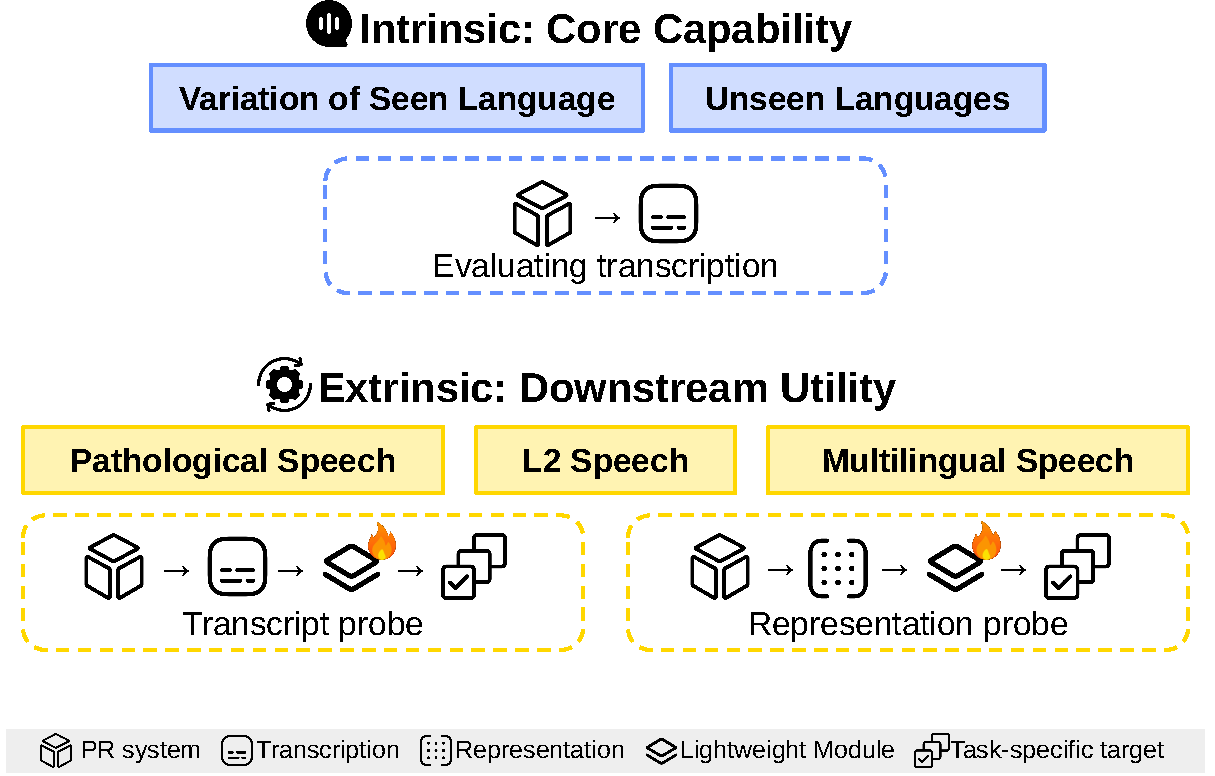
\includegraphics[width=0.92\linewidth]{figures/phonebench_tasks.pdf}
  \caption{\bench is the first open-source benchmark for phone recognition systems, covering intrinsic and extrinsic evaluations, i.e., transcription task and downstream task performance.}
  \label{fig:phonebench-design}
  \vspace{-1em}
\end{figure}

% Easy (but limited) fix of current eval: data & metric
PR models have scaled substantially to cover diverse linguistic settings (see \autoref{ss:bg-pr-system}), yet existing evaluations remain difficult to compare across studies. 
% Most prior work evaluates PR by comparing predicted transcriptions with gold labels. 
For example, models often differ in language coverage and phone inventories \cite{zipa}, and evaluation metrics are not standardized \cite{powsm}. 
A common response has been to fix a metric \cite{taguchi23_interspeech, powsm} and expand the number of test datasets to mitigate bias \cite{zipa}. Yet this approach scales poorly due to the scarcity of phonetically transcribed data. 
% Why we need downstream tasks -- transcription error rate alone isn't reliable
Moreover, transcription error rates do not necessarily reflect a model's phonetic capabilities or practical utility. 
Error rates in PR are inherently noisier than in ASR, as phones, unlike lexical units, correspond to a lower-level, articulatorily defined abstraction of the acoustic signal.

Furthermore, the link between transcription accuracy and downstream performance is often assumed rather than empirically proven. In practice, models leverage phonetic information via two channels: explicit transcriptions and latent internal representations. The latter are especially potent, as they encode rich phonetic cues (see \autoref{ss:bg-phonetic-info}). Consequently, metrics based solely on transcription error fail to capture the full utility and nuanced quality of these representations.


% Propose phonebench
Therefore, we propose \textbf{\bench} to fairly benchmark \textbf{P}hone \textbf{R}ealization \textbf{i}n \textbf{S}peech \textbf{M}odels.
\bench assesses PR systems\footnote{Any pipeline that converts speech into phonetic units.} intrinsically through transcription error, and extrinsically through utility in clinical, educational, and multilingual speech tasks using generated transcriptions and hidden representations. 
\bench applies to PR systems ranging from specialized PR models to general speech-to-text (S2T) systems, including Large Audio Language Models (LALMs), which are increasingly used for general speech tasks despite limited evaluation of their phonetic abilities \citep{peng2024slmsurvey, arora2025landscape}. 

% Contribution & goal
\bench is the first open-source benchmark for PR systems, for which code, evaluation recipes, and datasets are released, where licensing permits.
With its reproducible and expandable framework, \bench supports researchers in understanding model behavior and training strategies, and helps practitioners make informed model choices. 
We evaluate a broad range of PR systems and find that:
(i) \textbf{language exposure matters}: seen languages benefit from familiar patterns, unseen from multilingual training;
(ii) \textbf{data and architecture shape performance}: broad, diverse coverage improves results, while encoder-CTC architectures are more stable;
(iii) \textbf{LALMs lag behind specialized PR models}.

Ultimately, our goal is to establish a common evaluation basis to drive progress toward PR systems that capture robust and generalizable phonetic information across resource conditions.